%% Journal of Open Research Software Latex template -- Created By Stephen Bonner and John Brennan, Durham Universtiy, UK.

\documentclass{jors}
\usepackage{amsmath, amssymb}
\usepackage{cite}
\usepackage{graphicx}
\graphicspath{ {images/} }

%% Set the header information
\pagestyle{fancy}
\definecolor{mygray}{gray}{0.6}
\renewcommand\headrule{}
\rhead{\footnotesize 3}
\rhead{\textcolor{gray}{UP JORS software Latex paper template version 0.1}}

\begin{document}

{\bf Software paper for submission to the Journal of Open Research Software} \\

Please submit the completed paper to: editor.jors@ubiquitypress.com

\rule{\textwidth}{1pt}

\section*{(1) Overview}

\vspace{0.5cm}

\section*{Title}
spinsim: a GPU optimised solver of spin half and spin one quantum systems

\section*{Paper Authors}
1. Tritt, Alex;\\
2. Morris, Joshua;\\
3. Hochstetter, Joel;\\
4. Anderson, R. P.;\\
5. Saunderson, James;\\
6. Turner, L. D.;\\

\section*{Paper Author Roles and Affiliations}
1. School of Physics \& Astronomy, Monash University, Victoria 3800, Australia.\\
	Primary author of the released packages.\\
2. School of Physics \& Astronomy, Monash University, Victoria 3800, Australia.\\
	Present address: Faculty of Physics, University of Vienna, 1010 Vienna, Austria.\\
	Author of first version of code.\\
3. School of Physics \& Astronomy, Monash University, Victoria 3800, Australia.\\
	Present address: School of Physics, University of Sydney, NSW 2006, Australia.\\
	Optimization and extension to spin one of first version of code.\\
4. School of Molecular Sciences, La Trobe University, PO box 199, Bendigo, Victoria 3552, Australia.\\
	Original conception of first version of code.\\
5. Department of Electrical and Computer Systems Engineering, Monash University, Victoria 3800, Australia.\\
	Advice on numerical analysis.\\
6. School of Physics \& Astronomy, Monash University, Victoria 3800, Australia.\\
	Original conception of released version of algorithm.

\section*{Abstract}
	\texttt{spinsim} is a \emph{python} package that simulates spin half and spin one quantum mechanical systems following a time dependent Shroedinger equation. It makes use of \texttt{numba.cuda} \cite{lam_numba_2015}, which is an \emph{LLVM} (Low Level Virtual Machine) \cite{lattner_llvm_2004} compiler, and other optimisations, to allow for fast and accurate evaluation on \emph{Nvidia Cuda} \cite{nickolls_scalable_2008} compatible systems using GPU parallelisation. \texttt{spinsim} is available for installation on \emph{PyPI}, and the source code is available on \emph{github}. The initial use case for the package will be to simulate quantum sensing-based Bose Einstein condensate (BEC) experiments for the Monash University School of Physics and Astronomy spinor BEC lab, but we anticipate it will be useful in simulating any range of spin half or spin one quantum systems with time dependent Hamiltonians that cannot be solved analytically. These appear in the fields of nuclear magnetic resonance (NMR), nuclear quadrupole resonance (NQR) and magnetic resonance imaging (MRI) experiments and quantum sensing, and with the spin one systems of nitrogen vacancy centres (NVCs) and BECs.

\section*{Keywords}
Time dependent Schroedinger equation; Spin one; Spin half; Integrator; GPU; Solver; python; numba;

\section*{Introduction}
\subsection*{Motivation}
	Ultracold rubidium atoms have proven their effectiveness in state of the art technologies in quantum sensing \cite{degen_quantum_2017}, the use of quantum mechanics to make precise measurements of small signals. The rotation of these atoms can be modelled as quantum spin systems, which is the quantum mechanical model for objects with angular momentum. The simplest spin system, spin half (also referred to as a qubit), is quantised into just two quantum spin levels, and this describes the motion of some fundamental particles such as electrons. However, systems more practical for sensing, such as ultracold rubidium atoms, are more accurately described as a spin one quantum system (also referred to as a quitrit), which is quantised into three quantum spin levels.
	
	The design of sensing protocols requires many steps of verification, including simulation. This is especially important, since running real experiments can be expensive and time consuming, and thus it is more practical to debug such protocols quickly and cheaply on a computer. In general, any design of experiments using spin systems could benefit from a fast, accurate method of simulation.

	In the past, the spinor Bose Einstein condensate (spinor BEC) lab at Monash University used an in-house, \emph{cython} based script \texttt{AtomicPy} \cite{morris_qcmonkatomicpy_2018}, on which this package is based, and standard differential equation solvers (such as \emph{Mathematica}'s function \texttt{NDSolve}) to solve the Schroedinger equation for quantum sensing spin systems. These spin one systems  are sometimes approximated to spin half for a faster execution time, at the cost of modelling all effects of the system. However, these methods are not completely optimised for our use case, and therefore come with some issues.

	First, while the execution time for these solvers is acceptable for running a small number of experiments, for certain experiments involving large arrays of independent atom clouds (which require many thousands of simulations to be run), this time accumulates to the order of many hours.

	Second, the Schroedinger equation has the geometric property of being norm persevering. In other words, the time evolution operator for a system between two points in time must be unitary. As such, numerical solutions to the Schroedinger equation should also preserve this property. For many numerical methods like those in the Runge Kutta family, the approximations used might not be norm preserving, and the evaluated quantum state may diverge towards an infinite norm, or converge to zero if run for many iterations.

	Third, our system (and similar spin systems) can be very oscillatory. In standard conditions for our application, the expected spin projection of a system that we want to solve for can rotate in physical space (alternatively viewed as a point rotating around an abstract object known as a \emph{Bloch sphere}) at a rate of 700kHz. Standard integration methods require very small time steps in order to accurately depict these oscillations. For instance, we found that the integration method used by \emph{AtomicPy} has an accuracy of only order \(10^{-2}\) when the integration time step is set to the small value of 10ns.

\section*{Implementation and architecture}
	\subsection*{Mathematical methods}
		\subsubsection*{Background}
			In general, \texttt{spinsim} solves the Schroedinger equation,

			\begin{align}
				\frac{\mathrm{d}}{\mathrm{d}t}\psi(t) &= -iH(t)\psi(t),
			\end{align}

			where \(i^2 = -1\), the state \(\psi(t) \in \mathbb{C}^N\) a time dependent, \(N\) dimensional, unit complex vector, and the Hamiltonian \(H(t) \in \mathbb{C}^{N \times N}\) is a time dependent \(N \times N\) complex Hermitian matrix. Here \(N\) is the number spin levels in the quantum system, so spin half is the \(N = 2\) case, and spin one refers to the \(N = 3\) case. Rather than being represented by standard coodintaes in \(\mathbb{C}^{N \times N}\), in \texttt{spinsim} the Hamiltonian \(H(t)\) is instead represented with respect to a choice of basis for the corresponding Lie Algebra, \(\mathfrak{su}(N)\). For example, when set to spin half mode, the \texttt{spinsim} package solves the time dependent Schroedinger equations of the form

			\begin{align}
				\frac{\mathrm{d}}{\mathrm{d}t}\psi(t) = -i 2\pi (f_x(t) J_x + f_y(t) J_y + f_z(t) J_z) \psi(t),
			\end{align}

			where \(i^2 = -1\), \(\psi(t) \in \mathbb{C}^2\), and the spin half spin projection operators are given by

			\begin{align}
				J_x &= \frac12\begin{pmatrix}
					0 & 1 \\
					1 & 0
				\end{pmatrix},
				&J_y &= \frac12\begin{pmatrix}
					0 & -i \\
					i &  0
				\end{pmatrix},
				&\textrm{and }J_z &= \frac12\begin{pmatrix}
					1 &  0 \\
					0 & -1
				\end{pmatrix}.
			\end{align}

			The energy source \(f\) that represents the time dependent Hamiltonian \(H(t)\), is the collection of energy functions \(f_x(t), f_y(t), f_z(t)\), with \(t\) in units of s and \(f\) in units of Hz that control the dynamics of the system. The user must define a method that returns a sample of these source functions when a sampling time is input. In physical terms, these functions could represent the \(x,y,z\) components of a magnetic field applied to a magnetically sensitive.

			Similarly, when \texttt{spinsim} is set to spin one mode, it can solve the Schroedinger equation of the form

			\begin{align}
				\frac{\mathrm{d}}{\mathrm{d}t}\psi(t) = -i 2\pi (f_x(t) J_x + f_y(t) J_y + f_z(t) J_z + f_q(t) Q) \psi(t).
			\end{align}

			where now \(\psi(t) \in \mathbb{C}^3\), and the spin one operators are given by

			\begin{align}
				J_x &= \frac{1}{\sqrt{2}}\begin{pmatrix}
					0 & 1 & 0 \\
					1 & 0 & 1 \\
					0 & 1 & 0
				\end{pmatrix},&
				J_y &= \frac{1}{\sqrt{2}}\begin{pmatrix}
					0 & -i &  0 \\
					i &  0 & -i \\
					0 &  i &  0
				\end{pmatrix},\\
				J_z &= \begin{pmatrix}
					1 & 0 &  0 \\
					0 & 0 &  0 \\
					0 & 0 & -1
				\end{pmatrix},&
				\textrm{and }Q &= \frac{1}{3}\begin{pmatrix}
					1 &  0 & 0 \\
					0 & -2 & 0 \\
					0 &  0 & 1
				\end{pmatrix}.
			\end{align}

			The matrices \(J_x, J_y, J_z\) are regular spin operators, and \(Q\) is a quadrupole operator. Note that \(Q\) is proportional to \(Q_{zz}\) as defined by Hamley et al \cite{hamley_spin-nematic_2012}, and \(Q_0\) as defined by Di et al \cite{di_dipolequadrupole_2010}.

		\subsubsection*{Parallelisation}
			Given that \(\psi(t)\) is a unit vector, it is possible to write \(\psi(t)\) in terms of a unitary transformation \(U(t, t_0)\) of the state \(\psi(t_0)\), for any time \(t_0\). In other words, for any \(t_0,t \in \mathbb{R}\), there is a unitary transformation \(U(t, t_0)\) such that
			
			\begin{align}
				\psi(t) &= U(t, t_0)\psi(t_0).
			\end{align}
			
			This means that a time series for the state of the system can be evaluated by evaluating the time evolution operator between each of the sample times. Consider quantising time with
			\begin{align}
				t_k &= t_0 + \mathrm{D}t\cdot k,
			\end{align}

			where \(\mathrm{D}t\) is the time step of the time series (in contrast to \(\mathrm{d}t\), a smaller time step for integration). If we define

			\begin{align}
				\psi_k = \psi(t_k)\textrm{ and}\\
				U_k = U(t_{k}, t_{k-1}),
			\end{align}
			
			then the time series of states \(\psi_k\) and time evolution operators \(U_k\) satisfies

			\begin{align}
				\psi_k &= U_k\psi_{k-1}\label{eq:integration_compilation}
			\end{align}

			This presents an opportunity for parallelism. While each of the \(\psi_k\) must be evaluated sequentially, the value of the \(U_k\) is independent of the value of any \(\psi_{k_0}\), or any other \(U_{k_0}\). This means that the time evolution operators \(U_k\) can all be calculated in parallel, and it allows \texttt{spinsim} to use GPU parallelisation on the level of time sample points, so a speed up is achieved even if just a single simulation is run.

			In summary, \texttt{spinsim} splits the time evolution of the full simulation into time evolution \(U_k\) within small time intervals \([t_{k - 1}, t_{k}]\), which are each calculated massively in parallel on a GPU. When all the \(U_k\) are calculated, the CPU then multiplies the \(U_k\) together (a comparatively less demanding job than calculating them) using Equation \eqref{eq:integration_compilation} to determine the \(\psi_k\).

		\subsubsection*{Rotating frame}
			If the rotating frame option is selected, the \(U_k\) are first calculated within a rotating frame of reference as \(U^r_k\), which, in some situations, reduces the size of the source functions used in the calculation, increasing accuracy. The rotation speed of the rotating frame is calculated locally for each parallel time step \(U_k\), and only for rotations around the \(z\) axis. The rotating from source functions \(f^r_x, f^r_y, f^r_z,\) and \(f^r_q\) are related to the source function from the user input via
			
			\begin{align}
				f^r_x(t) + if^r_y(t) &= e^{-i 2\pi f_r t}(f_x(t) + if_y(t)),\\
				f^r_z(t) &= f_z(t) - f_r\textrm{, and}\\
				f^r_q(t) &= f_q(t), \textrm{ for spin one.}
			\end{align}
			
			Where \(f_r = f_z(t_k + \frac12\mathrm{D}t)\) is sampled the midpoint value of the source over the interval \([t_{k - 1}, t_k]\). This, assuming that a midpoint sample is representative of an average value over the time interval, decreases the magnitude of \(f_z(t)\), while leaving the other source components at an equivalent magnitude. The rotation is then applied to obtain the lab frame time evolution operator \(U_k\) via
			
			\begin{align}
				U_k &= \exp(-i 2 \pi f_r J_z \mathrm{D}t) U^r_k.
			\end{align}

			Specifically, this relationship is

			\begin{align}
				U_k &= \begin{pmatrix}
					e^{-i 2\pi f_r \mathrm{D}t} & 0 & 0\\
					0 & 1 & 0\\
					0 & 0 & e^{i 2\pi f_r \mathrm{D}t}
				\end{pmatrix} U^r_k, \textrm{ for spin one, and}\\
				U_k &= \begin{pmatrix}
					e^{-i \pi f_r \mathrm{D}t} & 0\\
					0 & e^{i \pi f_r \mathrm{D}t}
				\end{pmatrix} U^r_k, \textrm{ for spin half.}
			\end{align}

			It is a common technique in solving quantum mechanical problems to enter rotating frames, and their more abstract counterparts of interaction pictures \cite{j_j_sakurai_jun_john_modern_1994}. Note that this is typically done in conjunction with the Rotating Wave Approximation (RWA), which is an assumption that the oscillatory components of \(f^r_x, f^r_y, f^r_z,\) and \(f^r_q\) on an average of many cycles do not have a large contribution to time evolution of the solution and can be ignored. In some cases, this allows for analytic solutions to the approximate quantum system to be obtained. Note that the RWA is \emph{not} invoked in \texttt{spinsim}, as doing this would reduce the accuracy of simulation results, defeating our purpose of using a rotating frame.
			
		\subsubsection*{Magnus based integration method}
			The integration method used in \texttt{spinsim} is the CF4 method from Auer et al \cite{auer_magnus_2018}. Each of the \(U_k\) are split into products of time evolution operators between times separated by a smaller timestep, that is,
			
			\begin{align}
				U(t_k, t_{k-1}) &= U(t_k, t_k - \mathrm{d}t) \cdots U(t_{k-1} + 2\mathrm{d}t, t_{k-1} + \mathrm{d}t) U(t_{k-1} + \mathrm{d}t, t_{k-1})\\
				U_k &= u^k_{L-1} \cdots u^k_0,\textrm{, where}\\
				u^k_{L-1} &= U(t_0 + (k - 1)\mathrm{D}t + (l + 1)\mathrm{d}t, t_0 + (k - 1)\mathrm{D}t + l\mathrm{d}t)
			\end{align}

			with \(\mathrm{d}t\) being the integration level, (ie, fine) time step. Note that the timesteps are related to each other by \(\mathrm{D}t = L\mathrm{d}t\), where \(L\in\mathbb{N}\).

			The CF4 method is used to calculate each individual \(u^k_l\). Let the fine sample time be given by \(t_f = l\mathrm{d}t + t_k\). Then as part of the CF4 method, the source functions are sampled at particular times based on the second order Gauss-Legendre quadrature, given by
			
			\begin{align}
				t_1 &= t_f + \frac12 \mathrm{d}t\left(1 - \frac{1}{\sqrt{3}}\right)\textrm{, and}\\
				t_2 &= t_f + \frac12 \mathrm{d}t\left(1 + \frac{1}{\sqrt{3}}\right).
			\end{align}

			Now, let
			\begin{align}
				f(t_1) &= (f_x(t_1), f_y(t_1), f_z(t_1), f_q(t_1))\textrm{, and}
				f(t_2) &= (f_x(t_2), f_y(t_2), f_z(t_2), f_q(t_2)).
			\end{align}
			
			The fine time evolution operator can then be calculated using
			
			\begin{align}
				g_1 =& (g_{1,x}, g_{1,y}, g_{1,z}, g_{1,q})\\
				=& 2 \pi \mathrm{d}t \left(\frac{3 + 2 \sqrt{3}}{12} f(t_1) + \frac{3 - 2 \sqrt{3}}{12} f(t_2)\right)\textrm{, and}\\
				g_2 =& (g_{2,x}, g_{2,y}, g_{2,z}, g_{2,q})\\
				=& 2 \pi \mathrm{d}t \left(\frac{3 - 2 \sqrt{3}}{12} f(t_1) + \frac{3 + 2 \sqrt{3}}{12} f(t_2)\right)\textrm{, so}\\
				u =& \exp(-i \left( g_{2,x} J_x + g_{2,y} J_y + g_{2,z} J_z + g_{2,q} Q\right))\\
				&\cdot\exp(-i \left( g_{1,x} J_x + g_{1,y} J_y + g_{1,z} J_z + g_{1,q} Q\right)).
			\end{align}

		\subsubsection*{Exponentiator}
			For all exponentiation, the exponentiator computes the matrix exponential
			
			\begin{align}
				E(g) &= E(g_x, g_y, g_z, g_q)\\
				&= \exp(-i (g_x J_x + g_y J_y + g_z J_z + g_q Q)), \textrm{ with}
			\end{align}
			
			For spin half, the default exponentiator is in an analytic form. For spin one, an exponentiator based on the Lie Trotter product formula \cite{moler_nineteen_2003} is used. Specifically, the exponential can be approximated as, for large \(\tau\),

            \begin{align*}
                E(g) &= \exp(-ig_x J_x - ig_y J_y - ig_z J_z - ig_q Q)\\
                &= \exp(2^{-\tau}(-ig_x J_x - ig_y J_y - ig_z J_z - ig_q Q))^{2^\tau}\\
                &\approx (\exp(-i(2^{-\tau} g_x) J_x) \exp(-i(2^{-\tau} g_y) J_y) \exp(-i(2^{-\tau} g_z J_z + (2^{-\tau} g_q) Q)))^{2^\tau}\\
                &= \begin{pmatrix}
                    \frac{e^{-i\left(Z + \frac{Q}{3}\right)}(c_X + c_Y - i s_Xs_Y)}{2} & \frac{e^{i\frac{2Q}{3}} (-s_Y -i c_Y s_X)}{\sqrt{2}} & \frac{e^{-i\left(-Z + \frac{Q}{3}\right)}(c_X - c_Y + i s_Xs_Y)}{2} \\
                    \frac{e^{-i\left(Z + \frac{Q}{3}\right)} (-i s_X + c_X s_Y)}{\sqrt{2}} & e^{i\frac{2Q}{3}} c_X c_Y & \frac{e^{-i(Z - \frac{Q}{3})} (-i s_X - c_X s_Y)}{\sqrt{2}} \\
                    \frac{e^{-i\left(Z + \frac{Q}{3}\right)}(c_X - c_Y - i s_Xs_Y)}{2} & \frac{e^{i\frac{2Q}{3}} (s_Y -i c_Y s_X)}{\sqrt{2}} & \frac{e^{-i\left(-Z + \frac{Q}{3}\right)}(c_X + c_Y + i s_Xs_Y)}{2}
                \end{pmatrix}^{2^\tau}\\
                &= T^{2^\tau},
            \end{align*}

			with

            \begin{align*}
                X &= 2^{-\tau}g_x,\\
                Y &= 2^{-\tau}g_y,\\
                Z &= 2^{-\tau}g_z,\\
                Q &= 2^{-\tau}g_q,\\
                c_{\theta} &= \cos(\theta),\\
                s_{\theta} &= \sin(\theta).
            \end{align*}
        
			Once \(T\) is calculated, it is then recursively squared \(\tau\) times to obtain \(E(g)\). The approach used for spin one exponentiation means that the package cannot solve arbitrary spin one quantum systems, as that would require the ability to exponentiate a point in the full, 8 dimensional Lie algebra of \(\mathfrak{su}(3)\), rather than just the four dimensional subspace spanned by the subalgebra \(\mathfrak{su}(2)\) spanned by \(\{J_x, J_y, J_z\}\), and the single quadratic operator \(Q\). Including the full algebra could be possible as a feature update if there is demand for it, though just including this subspace is sufficient for our application, and many others, and has the advantage of being able to use this faster, more specialised method of matrix exponentiation.

			Note that, the methods for both spin half and spin one use analytic forms of exponentials to construct the result, meaning that all calculated time evolution operators are unitary. This guarantees that the results of \texttt{spinsim} maintain unitary. 

	\subsection*{Software architecture}
		\subsubsection*{Integrator architecture}
			The integrator in the \texttt{spinsim} package calls a \texttt{numba.cuda.jit()}ed kernel to be run on a \emph{Cuda} capable \emph{Nvidia} GPU in parallel, with a different thread being allocated to each of the \(U_k\). This returns when each of the \(U_k\) have been evaluated.
			
			The thread starts by calculating \(t_k\) and, if the rotating frame is being used, \(f_r\). The latter is done by sampling a (\texttt{numba.cuda.jit()}ed version of a) user provided \emph{python} function \(f\) describing how to sample the source Hamiltonian. The code then loops over each fine time step \(\mathrm{d}t\) to calculate the fine time evolution operators \(u^k_l\).
			
			Within the loop, the integrator enters a device function (ie a GPU subroutine, which is inline for speed) to sample \(f(t)\), as well as calculate \(e^{-i 2 \pi f_r t}\), at the sample times needed for the integration method. After this, it enters a second device function, which makes a rotating wave transformation as needed in a third device function, before calculating \(g\) values, and finally taking the matrix exponentiation in a fourth device function. \(u^k_l\) is premultiplied to \(U^r_k\) (which is initialised to \(1\)), and the loop continues.
			
			When the loop has finished, if the rotating frame is being used, \(U^r_k\) is transformed to \(U_k\) as in Equation \eqref{eq:integration_compilation}, and this is returned. Once all threads have executed, the state \(\psi_k\) is calculated in a (CPU) \texttt{numba.jit()}ed function from the \(U_k\) and an initial condition \(\psi_{\mathrm{init}}\).
	
	
		\subsubsection*{Compilation of integrator}
			The \texttt{spinsim} integrator is constructed and compiled just in time, using \texttt{numba.cuda.jit()}. The particular device functions used are not predetermined, but are instead chosen based on user input to decide a closure. This structure has multiple advantages. First, the source function \(f\) is provided by the user as a plain python function (that must be \texttt{numba.cuda.jit()} compatible). This allows users to define \(f\) in a way that compiles and executes fast, does not put many restrictions on the form of the function, and returns the accurate results of analytic functions (compared to the errors seen in interpolation). Compiling the simulator also allows the user to set metaparameters, and choose the features they want to use, in a way that does not require experience with the \texttt{numba.cuda} library. This was especially useful for running benchmarks comparing old integration methods to the new ones, like CF4. The default settings should be optimal for most users, although tuning the values of \emph{Cuda} metaparameters \texttt{max\_registers} and \texttt{threads\_per\_block} could improve performance for GPUs with a differing number of registers and \emph{Cuda} cores to the mobile GTX1070 mainly used in testing here. Finally, just in time compilation also allows the user to select a target device other than \emph{Cuda} for compilation, so the simulator can run, using the same algorithm, on a multicore CPU in parallel instead of a GPU, if the user so chooses.
			
			This functionality is interfaced through an object of class \texttt{spinsim.Simulator}. The \emph{Cuda} kernel is defined as per the user’s instructions on construction of the instance, and it is used by calling the method \texttt{spinsim.Simulator.evaluate()}, which returns a results object including the time, state, time evolution operator, and expected spin projection (that is, Bloch vector). Note that the expected spin projection is calculated as a lazy parameter if needed, rather than returned by the simulator object.

\section*{Quality control}
	\subsection*{Benchmarks}
		\subsubsection*{Speed}
			Benchmarks were performed using \texttt{sense.sim.benchmark}, by comparing evaluation speed of typical spin one sensing experiments on different devices. This is shown in Figure \ref{fig:benchmark_device_aggregate}. The integration code was compiled by \texttt{numba} for single core CPUs, multicore CPUs, and \emph{Nvidia Cuda}, and run on different devices. These devices are,
			\begin{itemize}
				\item {} 
				Intel Core i7-8750H, a 6 core laptop processor released in 2018. Run with 16GiB of RAM. Air cooled (laptop fan). Base clock speed of 2.2GHz.

				\item {} 
				AMD Ryzen 7 5800X, an 8 core desktop processor released in 2020. Run with 32GiB of RAM. Liquid cooled. Base clock speed of 3.8GHz.

				\item {} 
				AMD Ryzen 9 5900X, a 12 core desktop processor released in 2020. Run with 32GiB of RAM. Air cooled. Base clock speed of 3.7GHz.

				\item {} 
				Nvidia GeForce GTX 1070, a 2048 \emph{Cuda} core laptop graphics processor released in 2016. Run with 8GiB of VRAM. Air cooled (laptop fan).

				\item {} 
				Nvidia GeForce RTX 3070, a 5888 \emph{Cuda} core desktop graphics processor released in 2020. Run with 8GiB of VRAM. Air cooled.

				\item {} 
				Nvidia GeForce RTX 3080, an 8704 \emph{Cuda} core desktop graphics processor released in 2020. Run with 10GiB of VRAM. Air cooled.
			\end{itemize}

			\begin{figure}[h!]
				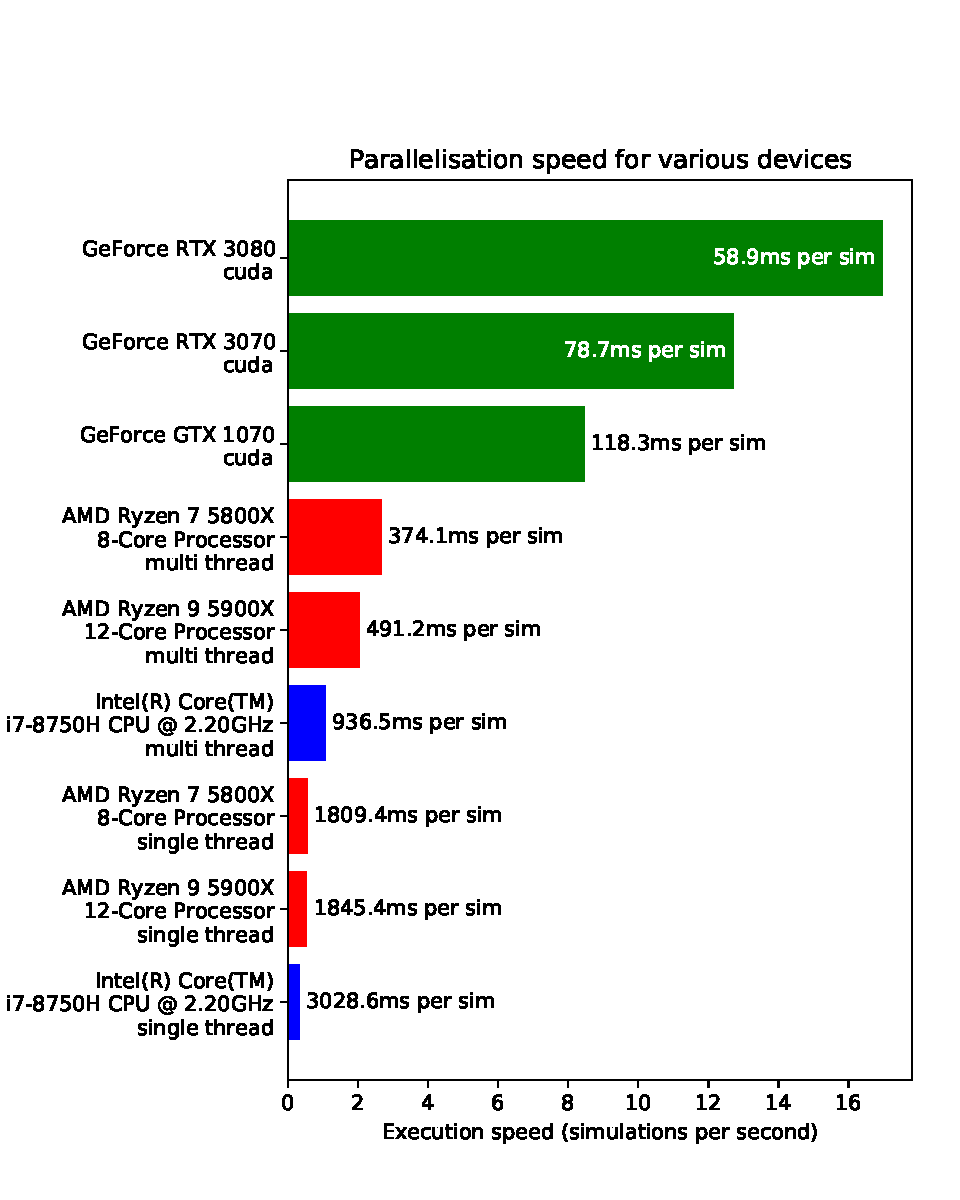
\includegraphics[scale=0.9]{benchmark_device_aggregate_publication.pdf}
				\caption{Evaluation speed of a typical spin one sensing experiment. Fine time step is 100ns, as determined to be ideal by the accuracy experiments. Experiments run for a duration of 100ms. Evaluation time is determined by an average of 100 similar experiments for each device.}
				\label{fig:benchmark_device_aggregate}
			\end{figure}

			This benchmark shows the benefit to using parallelisation when solving this problem. Moving from a 6 core processor to a 12 core processor doubles the execution speed. Moving from a single core processor to a GPU increases performance by well over an order of magnitude. As an aside, liquid cooling allows the 8 core processor to increase its boost clock and outperform the 12 core processor.

		\subsubsection*{Accuracy}
			Benchmarks were performed using \texttt{neural-sense.sim.benchmark} (where \texttt{neural-sense} \cite{alexander-tritt-monash_alexander-tritt-monashneural-sense_2020} is the quantum sensing package that \texttt{spinsim} was written for), by comparing state evaluations of many different typical sensing experiments and finding the mean error introduced when the fine (integration) time step is increased.

			\begin{figure}[h!]
				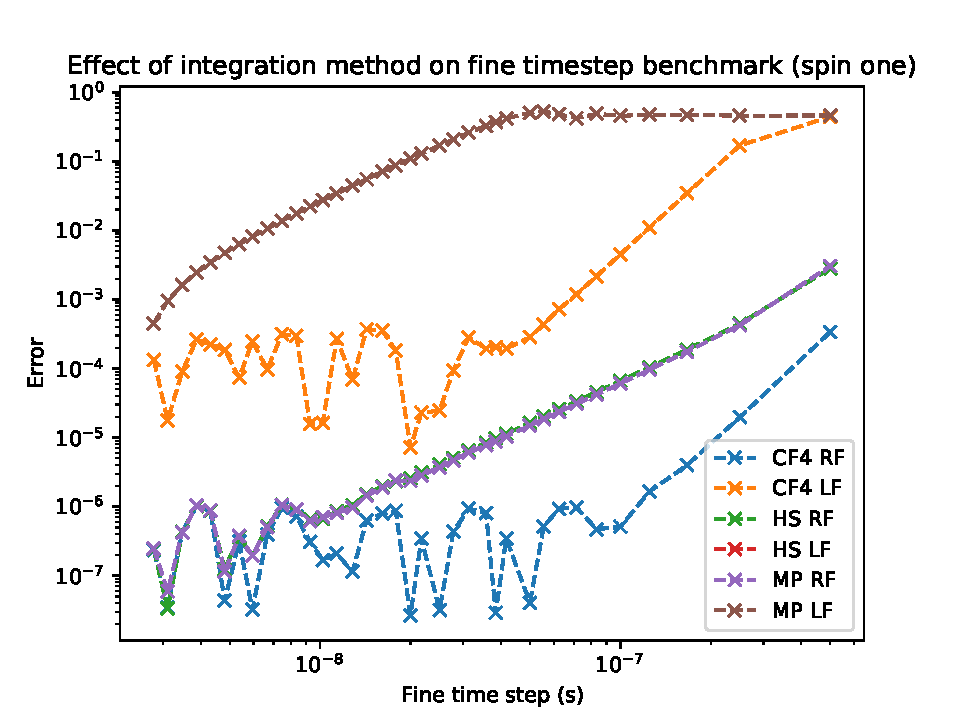
\includegraphics[scale=0.9]{benchmark_comparison_spin_one_publication.pdf}
				\caption{Fine time step benchmark for spin one systems. CF4 is the Magnus commutator free integrator, HS is the two sample exponential integrator used in \texttt{AtomicPy}, MP is a single sample exponential integrator, RF is use of the rotating frame, and LF is lab frame (no use of the rotating frame). HS and MP results are drawn on top of each other due to their similarities.}
				\label{fig:benchmark_comparison_spin_one}
			\end{figure}

			Figure \ref{fig:benchmark_comparison_spin_one} shows the performance of \texttt{spinsim} when running in spin one mode. This shows that both using the Magnus based CF4 method and moving into a rotating frame give significant increases to accuracy. The HS (half step) method in the lab frame, with a time step of 10ns was the method used by \texttt{AtomicPy}, the previous code used by the group for simulating spin systems. Compared to this, the best performing \texttt{spinsim} method is 5 orders of magnitude more accurate, while executing in a time 2 orders of magnitude faster.

			\begin{figure}[h!]
				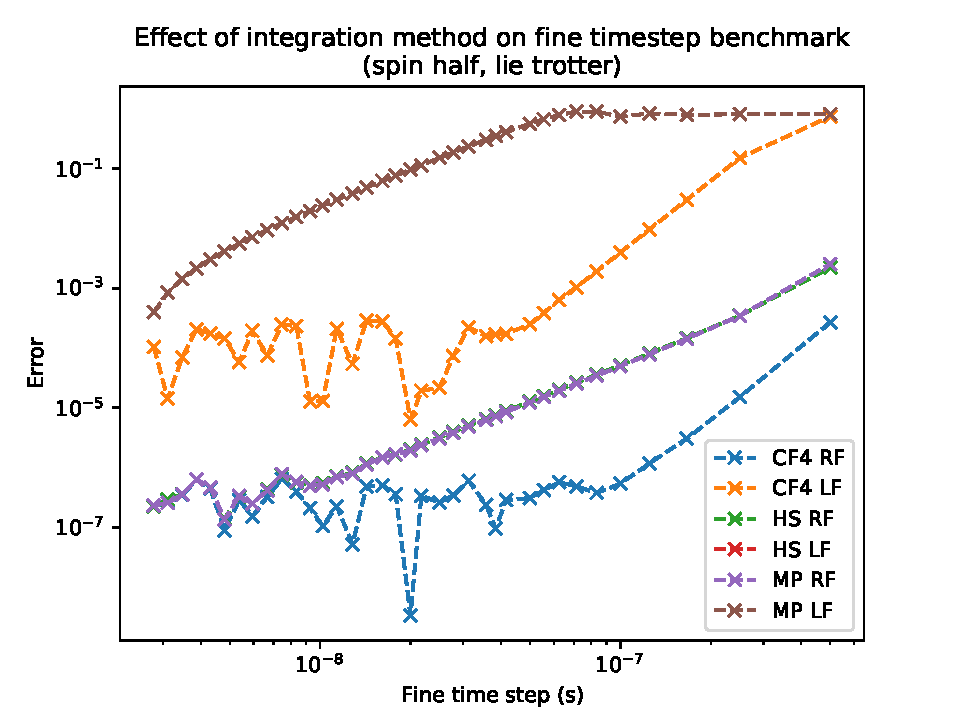
\includegraphics[scale=0.9]{benchmark_comparison_spin_half_lt_publication.pdf}
				\caption{Fine time step benchmark for spin half systems, using the Lie Trotter based exponentiator. CF4 is the Magnus commutator free integrator, HS is the two sample exponential integrator used in \texttt{AtomicPy}, MP is a single sample exponential integrator, RF is use of the rotating frame, and LF is lab frame (no use of the rotating frame). HS and MP results are drawn on top of each other due to their similarities.}
				\label{fig:benchmark_comparison_spin_half_lt}
			\end{figure}

			From Figure \ref{fig:benchmark_comparison_spin_half_lt}, one gets essentially the same accuracy for each method when working in spin half mode compared to spin one, if all else is kept constant.

			\begin{figure}[h!]
				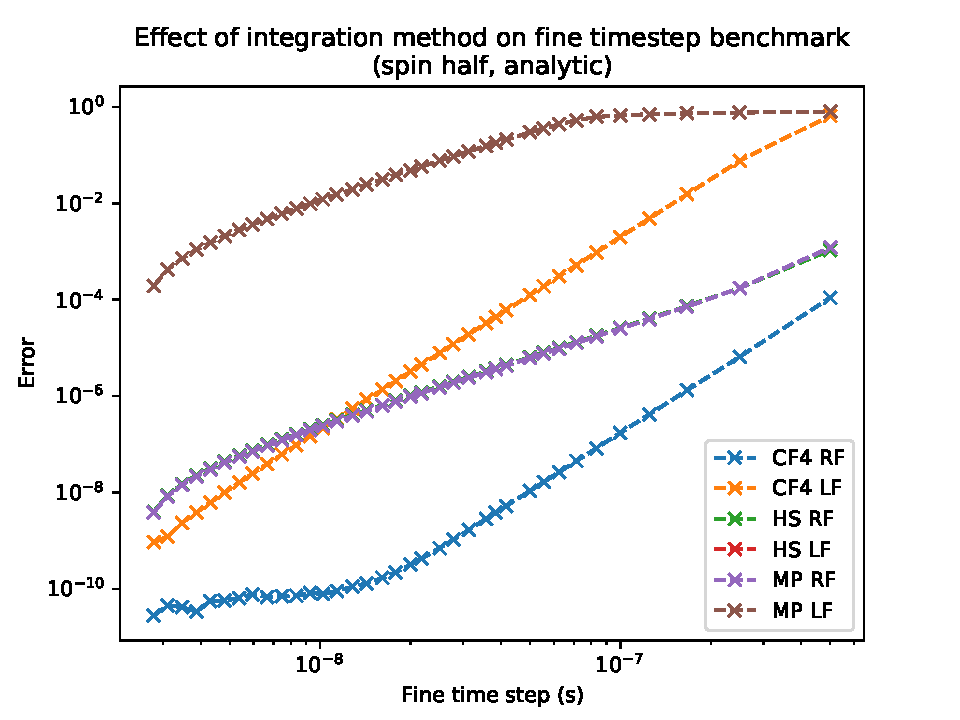
\includegraphics[scale=0.9]{benchmark_comparison_spin_half_a_publication.pdf}
				\caption{Fine time step benchmark for spin half systems, using the analytic based exponentiator. CF4 is the Magnus commutator free integrator, HS is the two sample exponential integrator used in \texttt{AtomicPy}, MP is a single sample exponential integrator, RF is use of the rotating frame, and LF is lab frame (no use of the rotating frame). HS and MP results are drawn on top of each other due to their similarities.}
				\label{fig:benchmark_comparison_spin_half_a}
			\end{figure}

			Figure \ref{fig:benchmark_comparison_spin_half_a} shows that the Lie Trotter based exponentiator does limit the maximum accuracy obtainable, and for spin half systems, one can increase accuracy further (and decrease execution time) by using an analytic based exponentiator.

		\subsubsection*{Comparison to alternatives}
			As mentioned before, compared to our previous code, \texttt{AtomicPy}, the best performing \texttt{spinsim} method is 5 orders of magnitude more accurate, while executing in a time 2 orders of magnitude faster.

			Another solver used by the lab group is \emph{Mathematica}'s \texttt{NDSolve}.

			We had planned to benchmark against some other popular generic solvers. One such solver was \texttt{qutip.sesolve()}, a solver in the popular quantum mechanics \emph{python} library, \texttt{QuTip} \cite{johansson_qutip_2013}. However, due to a known bug with the library’s dependencies, this was not installable on Windows 10, the operating system being used for testing, and so benchmarks for it could not be run. We also planned to benchmark accuracy against the generic solver \texttt{scipy.integrate.ivp\_solve()} in the \emph{python} library \texttt{SciPy} \cite{virtanen_scipy_2020}. However, using the same \texttt{get\_field} function as in the spin one benchmarks used for the \texttt{spinsim}, simulating with a fine time step of 500ns (the largest used during the \texttt{spinsim} benchmarks), we found that a single simulation ran in 153s, which is over three orders of magnitude slower than the most accurate \texttt{spinsim} simulations. This means that a generous projection for the time it would take to run the same benchmarks that \texttt{spinsim} runs in 11 minutes, using \texttt{scipy} would be over six days; for an integration package not designed for this problem (and would therefore likely be less accurate).

	\subsection*{Testing}
		The simulator as a whole has been functionally tested against well known analytic approximations of the behaviour spin systems. This was done for every combination of integrator settings possible when compiling the integrator. The system was benchmarked in terms of accuracy vs fine time step, again, using every possible combination of integrator settings. This confirms that no integrator diverges away from the limiting solution when the time step is decreased in magnitude. The Lie Trotter matrix exponentiator was tested separately from the full system, as well as benchmarked separately.

		These tests and benchmarks were run as part of the \texttt{neural\_sense} package. The simulator has also been used as part of the measurement protocol being developed there, and it has been tested as part of those algorithms as well.

		The kernel execution was profiled thoroughly, and changes were made to optimise VRAM and register usage and transfer. This was done specifically for the hardware of an Nvidia GTX1070, so one may get some performance increases by changing some GPU specific metaparameters when instantiating the \texttt{spinsim.Simulator} object.

		A good way to confirm that \texttt{spinsim} is functioning properly after an installation is to run the tutorial code provided and compare the outputs. Otherwise, one can run the benchmarks and simulation protocols in \texttt{neural\_sense.sim.benchmark}.

\section*{(2) Availability}
\vspace{0.5cm}
\section*{Operating system}
Developed on Windows 10. Tested on MacOS Big Sur.

\section*{Programming language}
Python (3.7 or greater)

\section*{Additional system requirements}
To use the (default) \emph{Nvidia Cuda} GPU parallelisation, one needs to have a \href{https://developer.nvidia.com/cuda-gpus}{\emph{Cuda} compatible \emph{Nvidia GPU}}. For \emph{Cuda} mode to function, one also needs to install the \href{https://developer.nvidia.com/cuda-toolkit}{\emph{Nvidia Cuda} toolkit}. If \emph{Cuda} is not available on the system, the simulator will automatically parallelise over multicore CPUs instead

\section*{Dependencies}
numba (0.50.1 or greater)\\
numpy (1.19.3)\\
matplotlib (for example code, 3.2)\\
neuralsense (for benchmark code)

\section*{List of contributors}

1. Alex Tritt\\
	School of Physics \& Astronomy, Monash University, Victoria 3800, Australia.\\
	Primary author of the released packages.\\
2. Joshua Morris\\
	School of Physics \& Astronomy, Monash University, Victoria 3800, Australia.\\
	Present address: Faculty of Physics, University of Vienna, 1010 Vienna, Austria.\\
	Author of first version of code.\\
3. Joel Hockstetter\\
	School of Physics \& Astronomy, Monash University, Victoria 3800, Australia.\\
	Present address: School of Physics, University of Sydney, NSW 2006, Australia.\\
	Optimization and extension to spin one of first version of code.\\
4. Russell P. Anderson\\
	School of Molecular Sciences, La Trobe University, PO box 199, Bendigo, Victoria 3552, Australia.\\
	Original conception of first version of code.\\
5. James Saunderson\\
	Department of Electrical and Computer Systems Engineering, Monash University, Victoria 3800, Australia.\\
	Advice on numerical analysis.\\
6. Lincoln D. Turner\\
	School of Physics \& Astronomy, Monash University, Victoria 3800, Australia.\\
	Original conception of released version of algorithm.

\section*{Software location:}

{\bf Archive}

\begin{description}[noitemsep,topsep=0pt]
	\item[Name:] Monash Bridges
	\item[Persistent identifier:] \textcolor{blue}{e.g. DOI, handle, PURL, etc.}
	\item[Licence:] BSD 3 Clause
	\item[Publisher:]  Alex Tritt
	\item[Version published:] 1.0.0
	\item[Date published:] \textcolor{blue}{dd/mm/yy}
\end{description}

{\bf Code repository}

\begin{description}[noitemsep,topsep=0pt]
	\item[Name:] GitHub
	\item[Persistent identifier:] https://github.com/alexander-tritt-monash/spinsim
	\item[Licence:] BSD 3 Clause
	\item[Date published:] 18/11/20
\end{description}

\section*{Language}

English.

\section*{(3) Reuse potential}

	\subsection*{Use potential and limitations}
		\texttt{spinsim} will be useful for any research group needing quick, accurate, and / or large numbers of simulations involving spin half or spin one systems. This is immediately relevant to developing new quantum sensing protocols with spin half and spin one systems. The package will be used in the context of Bose Einstein Condensate (BEC) magnetic sensing protocol design by our lab, both within and outside the project it was conceived for.

		This project is to be able to measure neural signals using BECs. The electrical pulses made by neurons are currently measured using electrical probes, which is intrusive and damages the cells. We instead propose to sense the small magnetic fields that these electrical currents produce. Rubidium BECs can potentially be made sensitive enough to these tiny magnetic fields that they can be measured by them. \texttt{spinsim} was written to simulate possible measurement protocols for this, showing the behaviour of the array of spin one atoms interacting with the magnetic fields of the neurons, control signals, and noise. The package is also now being used to simulate other BEC magnetometry experiments by the lab group.

		Another example of spin based magnetic field sensing is the use of Nitrogen Vacancy Centres (NVCs). These are spin one structures found in diamond doped with Nitrogen atoms. This leaves a vacancy in a position adjacent to the Nitrogen atom, which pairs of electrons occupy to obtain the spin one properties. Similar to BECs, NVCs can be placed and addressed in 2D arrays in order to take many samples in one measurement. A paper was only recently released covering simulation experiments of magnetic neural pulse sensing using NVCs \cite{parashar_axon_2020}, which is something that \texttt{spinsim} could be useful for.

		\texttt{spinsim} is designed to simulate small dimensional quantum systems, including large arrays of non-interacting spin systems. This means that it would not be able to integrate large arrays of entangled states or interacting particles. As a result, despite being fast at simulating qubits, it is inappropriate for the package to be used for quantum computing. In addition, \texttt{spinsim} is currently designed to integrate the time evolution of pure states only. This means that it may not be adequate for use in some Nuclear Magnetic Resonance (NMR) applications where relaxation \cite{veshtort_spinevolution_2006} is important (or other kinds of simulations involving decoherence).

		With these restrictions in mind, \texttt{spinsim} could be used for some simplified simulations in various areas of NMR. There are many atomic nuclei with spins of half (eg protons, Carbon 13) and, and fewer that have spins of one (eg Lithium 6, Nitrogen 14) \cite{fuller_nuclear_1976}, which, if relaxation and interactions between systems are not important for the application, \texttt{spinsim} could be used to simulate for spectroscopy experiments, for example. The inclusion of a quadrupole operator means that, with the same level of simplifications, \texttt{spinsim} should be able to simulate Nuclear Quadrupole Resonance (NQR) spectroscopy for spin one nuclei \cite{bain_nqr_2004}, such as Nitrogen 14, provided a suitable coordinate system is chosen. This technique measures energy level differences between levels split by electric field gradients, rather than static magnetic bias fields. Another possible use case could be for Magnetic Resonance Imaging (MRI) simulation and pulse sequence design. MRI uses measures the response of spins of an array of spin half protons to a spatially varying pulse sequence \cite{mckinnon_physics_1998}, which essentially just corresponds to many separate \texttt{spinsim} simulations of spins at different positions in space. While this package offers some advantages over state of the art simulators in the field \cite{kose_fast_2019}, with its use of quantum mechanics over classical mechanics, and its absence of rotating wave approximations, its parametrised pulse sequence definitions and geometric integrator, again, the lack of interacting particles and decoherence features are may limit its use in this area.

	\subsection*{Support}
		Documentation for \texttt{spinsim} is available on \href{https://spinsim.readthedocs.io/en/latest/}{\emph{Read the Docs}}. This documentation contains a thorough tutorial on how to use the package, and installation instructions.
		
		For direct support with the \texttt{spinsim} package, one can open an issue in the \emph{github} repository. One can also use this contact to suggest extensions to the package. \texttt{spinsim} is planned to be maintained by the Monash University spinor BEC lab into the future.

\section*{Acknowledgements}

Thank you to Hamish Taylor and Travis Hartley from the Monash University School of Physics and Astronomy spinor BEC lab, who have started using \texttt{spinsim} for their own projects and have given feedback of their user experience with the package.

\section*{Funding statement}

\textcolor{blue}{If the software resulted from funded research please give the funder and grant number.}

\section*{Competing interests}

The authors declare that they have no competing interests.

\bibliography{spinsim}{}
\bibliographystyle{vancouver}

\vspace{2cm}

\rule{\textwidth}{1pt}

{ \bf Copyright Notice} \\
Authors who publish with this journal agree to the following terms: \\

Authors retain copyright and grant the journal right of first publication with the work simultaneously licensed under a  \href{http://creativecommons.org/licenses/by/3.0/}{Creative Commons Attribution License} that allows others to share the work with an acknowledgement of the work's authorship and initial publication in this journal. \\

Authors are able to enter into separate, additional contractual arrangements for the non-exclusive distribution of the journal's published version of the work (e.g., post it to an institutional repository or publish it in a book), with an acknowledgement of its initial publication in this journal. \\

By submitting this paper you agree to the terms of this Copyright Notice, which will apply to this submission if and when it is published by this journal.


\end{document}
